\subsection{\color{ForestGreen}Rice's Theorem, Post's Correspondence Problem}
\subsubsection{Definitions}
\begin{itemize}
    \item Property of languages: A set of languages (e.g. CFL's).
    \item $\mathbf{L_P}$: the set of binary TM codes for TM’s $M$ such that $L(M)$ has property $P$.
    \item A \textbf{reduction} from language $L$ to language $L^\prime$ is an algorithm that takes a string $w$ and converts it to a string $x$, s.t. $x\in L^\prime \iff w \in L$. If such a reduction exists, write $\mathbf{L \leq_m L^\prime}$. We reduce a known hard problem to one we wish to show is at least as hard. 
    \item \textbf{Halting problem}: the set of pairs $(M,w)$ such that $w\in H(M)$, where $H(M)$ is the set of inputs $w$ s.t. $M$ halts whether or not it accepts. It is RE but not recursive.
    \item \textbf{Non-Halting problem}: The set of pairs $(M, w)$ such that TM $M$ started with input $w$ does not halt. It can be shown to be not RE by reducing $\bar L_u$ to it. 
\end{itemize}
\subsubsection{Results}
\begin{itemize}
    \item $L_u$ is RE, but not a recursive language i.e. it is undecidable. Why? If $L_u$ were recursive, we could design an algorithm for $L_d$, which is impossible. Reduce $L_d$ to $\bar L_u$ with $f(w) = w111w$, then $w \in L_d \iff w111w \in \bar L_u.$
    \item If $L$ is recursive, so is $\bar L: =\Sigma ^* -L$: construct $M^\prime$ for $\bar L$. 
    \begin{enumerate}
        \item $M^\prime$ has one final state $f$. 
        \item $M^\prime$ simulates $M$, but if $M$ enters an accepting state, $M^\prime$ halts without accepting.
        \item If $M$ halts without accepting, $M^\prime$ instead has a move taking it to state $f$. In state $f$, $M^\prime$ halts.
    \end{enumerate}
    \item If $L$ and $\bar L$ are RE, then $L$ is recursive. 
    \item If there is a reduction from $P_1$ to $P_2$  (i.e. $P_1 \leq_m P_2$), then
    \begin{itemize}
        \item $P_1$ is undecidable $\implies \; P_2$ is undecidable.
        \item $P_1$ is Non-RE $\implies \; P_2$ is Non-RE.
        \item $P_2$ is decidable $\implies \; P_1$ is decidable.
    \end{itemize}
    \item $L_e := \{M | L(M) = \varnothing\}$ is non-RE.
    \item $L_{ne} : = \{ M | L(M) \neq \varnothing \} $ is RE but not recursive.
    \end{itemize}
    
\subsubsection{Rice's Theorem}
There are two trivial properties $P$ for which $L_P$ is \textit{decidable}.
\begin{enumerate}
    \item The \textit{always-false property}, which contains no RE languages.
    \item The \textit{always-true property}, which contains all RE languages.
\end{enumerate}
For ever other property $P$, $L_P$ is \textit{undecidable.} Therefore, all problems  about TM's that involve only the language that the TM accepts are undecidable. E.g. whether the language accepted by a TM is empty, finite, a regular language, etc.

\subsubsection{Post's Correspondence Problem (PCP)}
PCP is undecidable. From PCP, we can prove many other non-TM problems undecidable.

An instance of PCP is a list of pairs of nonempty strings over some alphabet $\Sigma$.
Say $(w_1, x_1), (w_2, x_2), \hdots, (w_n, x_n).$ The answer is
“yes” $\iff \exists \{i_1,\hdots,i_k\}$ s.t. $w_{i_1}w_{i_2}...w_{i_n} = x_{i_1}x_{i_2}...x_{i_n}.$

\textbf{MPCP}: Same as PCP, but solution must start with first pair in the list.

To prove PCP undecidable, show $L_u \leq_m MPCP \leq_m PCP.$

    Only the following are  possible:
    \begin{enumerate}
        \item Both $L$ and $\bar L$ are recursive.
        \item Neither $L$ nor $\bar L$ is RE.
        \item $L$ is RE but not recursive,  and $\bar L$ is not RE.
        \item $\bar L$ is RE but not recursive, and $L$ is not RE.
    \end{enumerate}
    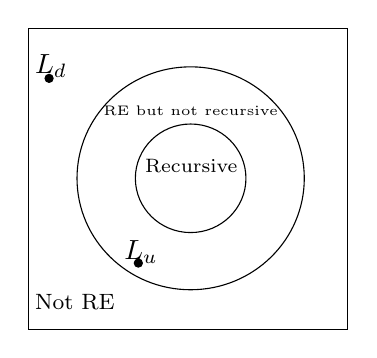
\begin{tikzpicture}[x=0.75pt,y=0.75pt,yscale=-1,xscale=1]
%uncomment if require: \path (0,300); %set diagram left start at 0, and has height of 300
%Shape: Rectangle [id:dp16952338970258785] 
\draw   (260,63.8) -- (414,63.8) -- (414,208.8) -- (260,208.8) -- cycle ;
%Flowchart: Connector [id:dp34086598366075627] 
\draw   (283.5,136.1) .. controls (283.5,106.44) and (308.01,82.4) .. (338.25,82.4) .. controls (368.49,82.4) and (393,106.44) .. (393,136.1) .. controls (393,165.76) and (368.49,189.8) .. (338.25,189.8) .. controls (308.01,189.8) and (283.5,165.76) .. (283.5,136.1) -- cycle ;
%Flowchart: Connector [id:dp43855418243619915] 
\draw   (311.61,136.1) .. controls (311.61,121.66) and (323.54,109.95) .. (338.25,109.95) .. controls (352.96,109.95) and (364.89,121.66) .. (364.89,136.1) .. controls (364.89,150.54) and (352.96,162.25) .. (338.25,162.25) .. controls (323.54,162.25) and (311.61,150.54) .. (311.61,136.1) -- cycle ;

%Shape: Circle [id:dp2730651255885239] 
\draw  [fill={rgb, 255:red, 0; green, 0; blue, 0 }  ,fill opacity=1 ] (268.1,87.95) .. controls (268.1,86.87) and (268.97,86) .. (270.05,86) .. controls (271.13,86) and (272,86.87) .. (272,87.95) .. controls (272,89.03) and (271.13,89.9) .. (270.05,89.9) .. controls (268.97,89.9) and (268.1,89.03) .. (268.1,87.95) -- cycle ;
%Shape: Circle [id:dp9402206153171893] 
\draw  [fill={rgb, 255:red, 0; green, 0; blue, 0 }  ,fill opacity=1 ] (311.1,176.95) .. controls (311.1,175.87) and (311.97,175) .. (313.05,175) .. controls (314.13,175) and (315,175.87) .. (315,176.95) .. controls (315,178.03) and (314.13,178.9) .. (313.05,178.9) .. controls (311.97,178.9) and (311.1,178.03) .. (311.1,176.95) -- cycle ;

% Text Node
\draw (262,75) node [anchor=north west][inner sep=0.75pt]   [align=left] {$\displaystyle L_{d}$};
% Text Node
\draw (305,165) node [anchor=north west][inner sep=0.75pt]   [align=left] {$\displaystyle L_{u}$};
% Text Node
\draw (262,190.8) node [anchor=north west][inner sep=0.75pt]   [align=left] {{\footnotesize Not RE}};
% Text Node
\draw (295,100) node [anchor=north west][inner sep=0.75pt]   [align=left] {{\tiny RE but not recursive}};
% Text Node
\draw (315,125.8) node [anchor=north west][inner sep=0.75pt]   [align=left] {{\scriptsize Recursive}};
\end{tikzpicture}



\subsubsection{CFG Ambiguity Problem}
CFG ambiguity problem is undecidable. Reduce PCP to CFG: Given a PCP instance consisting of lists $A = w_1, w_2,... ,w_k$ and $B = x_1 , x_2 ,..., x_k$, construct grammars for the two list languages, with variables $A$ and $B$.

For list $A$ we shall construct a CFG with $A$ as the only variable. The terminals are all the symbols of the alphabet used for this PCP instance plus a distinct set of index symbols $a_1,a_2, ..., a_k$ that represent the choices of pairs of strings in a solution to the PCP instance. That is the index symbol $a_i$ represents the choice of $w_i$ from the $A$ list or $x_i$ from the $B$ list. The productions for the CFG for the A list are, 
$A \xrightarrow{} w_1Aa_1 |...|w_kAa_k|w_1a_1|...|w_k a_k$. Call this grammar $G_A$ and its language $L_A$, analogously, $G_B$ and $L_B$. $L_A$ and $L_B$ are called \textbf{List Languages}. Combine $G_A$ and $G_B$ to form $G_{AB}$ which has the productions $S\xrightarrow{}A|B$ and all productions of $G_A$ and $G_B$. $G_{AB}$ is ambiguous $\iff$ the instance $(A,B)$ of PCP has a solution. 

The complement of a list language is also a CFL. Construct a deterministic PDA for the complement language:
\begin{itemize}
    \item Start with a bottom-of-stack marker. While PCP symbols arrive at the input, push them onto the stack. After the first index symbol arrives, start checking the stack for the reverse of the corresponding string
    \item $L_A^c \cup L_B^c = \Sigma^* \iff$ the PCP instance has no solution. So we have reduced PCP to "is a given CFL equal to all strings over its terminal alphabet?"
    \item Also undecidable: is a CFL a regular language? Same reduction from PCP: the CFL is regular $\iff L_A^c \cup L_B^c = \Sigma^*$
\end{itemize}
\subsubsection{Sample Exercise}
Show the set of all TM codes for TM's that fail to halt on at least one input is not RE.
Consider the simple reduction from the nonhalting problem. Given $(M,w)$, construct $M^\prime$ as follows:
\begin{enumerate}
    \item $M^\prime$ ignores its own input and simulates $M$ on $w$.
    \item If $M$ halts, $M^\prime$ halts on its own input. However, if $M$ never halts on $w$, then $M^\prime$ will never halt on its own input.
\end{enumerate}
As a result, $M^\prime$ fails to halt on at least one input (in fact, on all inputs) if $M$ fails to halt on $w$. If $M$ halts on $w$, then $M^\prime$ halts on all inputs.

